\chapter{Resultados}

La implementación del sistema dio como resultado un total de 178 videos tomados, de los cuales solo fueron procesados un total de 29 videos, la baja cantidad de videos procesados fue debido al tiempo de ejecución del sistema, además de que en algunos casos había que volver a procesar un mismo video varias veces, el sistema procesa entre 30 y 45 fotogramas por segundo lo cual se traduce en el mejor de los casos en 1.333 segundos procesar un segundo real de video.

Los 29 videos procesados dieron un total de 532 datos generados, con datos se realizaron los experimentos, los cuales comenzaron por el cálculo mostrado en la Sección SECCION, el uso de modelos implementados en la biblioteca Scikit Learn de Python para terminar con el uso de Tensor Flow implementado una red neuronal de capaz densas.

Para los experimentos los datos fueron separados por carril 0, 1 y 2, los cuales representan el primer carril, carril centrar y ultimo carril. Para cada uno de ellos tenemos 8 datos, 239 datos y 285 datos respectivamente, para el primer carril fueron omitidas las pruebas puesto que no se cuenta con datos suficientes.

Para todos los casos fue implementada la métrica de evaluación del promedio de error absoluto, con esto podemos darnos una idea de que tan precisa es nuestra predicción con los diferentes modelos implementados.


\section{Hardware utilizado}

El hardware utilizado fue una computadora física personal con las siguientes características:

\begin{itemize}
    \item CPU: Intel® Core™ i3-8100 CPU
    \item RAM: 32GB DDR4
    \item GPU: GeForce RTX 2070 SUPER
    \item OS: Ubuntu 20.04.2 LTS
\end{itemize}

\section{Regresión lineal para cálculo de la velocidad}

En la Sección \ref{cap:EstimacionVelocidad} mostramos el cálculo de la velocidad utilizando una regresión simple implementada utilizando solamente la formula básica de la velocidad, en estos experimentos se utilizó esta misma fórmula para el conjunto de datos creado con el sistema, utilizando solamente el carril central y el ultimo carril.

\subsection{Resultados Regresión lineal para cálculo de la velocidad}

En la Tabla \ref{tab:resultadosRLS} de resultados podemos notar que los mejores resultados están en el último carril con 5.86 K/H, mientras que el carril central tiene 7.74 K/H. Tomamos estos resultados como punto de referencia para mejorar las futuras predicciones, ya que estos no son tan buenos en comparación por ejemplo del margen de error del radar Bushnell utilizado.

\begin{table}[H]
    \centering
    \caption{Resultados usando regresión simple}
    \label{tab:resultadosRLS}
    \begin{tabular}{|l|l|l|}
    \hline
    \textbf{} & \textbf{M/S} & \textbf{K/H} \\ \hline
    \textbf{Carril Central} & 2.15 & 7.74 \\ \hline
    \textbf{Ultimo Carril}  & 1.63 & 5.86 \\ \hline
    \end{tabular}
\end{table}

\section{Scikit Learn}

Para el caso de la implementación de Scikit se utilizaron los siguientes modelos implementados en esta biblioteca:

\begin{itemize}
    \item Regresión Lineal
    \item Regresión de crestas
    \item Lasso (Operador de Selección y Contracción Mínima Absoluta)
    \item Regresión de la cresta bayesiana
    \item Regresión Elastic Net
    \item Regresión Random Forest
    \item Regresión de Máquina de Soporte Vectorial
\end{itemize}

Los experimentos con el uso de la biblioteca Scikit se realizaron un total de 800 veces, con estos resultados se obtuvo el valor mínimo, el valor máximo y el promedio de todos los experimentos.

\subsection{Carril central}

La tabla \ref{tab:resultadosScikitCarrilCentral} muestra los resultados para el carril central, en kilometros por hora.


\begin{table}[H]
    \centering
    \caption{Resultados para Carril Central}
    \label{tab:resultadosScikitCarrilCentral}
    \begin{tabular}{|l|l|l|l|l|l|l|l|} \hline
        & \textbf{RL} & \textbf{RC} & \textbf{Lasso} & \textbf{RCB} & \textbf{Elastic Net} & \textbf{RRF} & \textbf{RSVM} \\ \hline

        \textbf{MIN} & 1.246 & 1.256 & 1.271 & 1.253 & 1.278                & 1.433 & 1.598 \\ \hline
        \textbf{MAX} & 2.16 & 2.142 & 2.149 & 2.153 & 2.156                & 2.282 & 2.441 \\ \hline
        \textbf{Prom} & 1.692 & 1.696 & 1.699 & 1.696 & 1.699 & 1.829 & 1.962 \\ \hline
    \end{tabular}
\end{table}


\subsection{Ultimo Carril}

La tabla \ref{tab:resultadosScikitUltimoCarril} muestra los resultados para el ultimo carril, en kilometros por hora.


\begin{table}[H]
    \centering
    \caption{Resultados para Ultimo Carril}
    \label{tab:resultadosScikitUltimoCarril}
    \begin{tabular}{|c|l|l|l|l|l|l|l|} \hline
        & \textbf{RL} & \textbf{RC} & \textbf{Lasso} & \textbf{RCB} & \textbf{Elastic Net} & \textbf{RRF} & \textbf{RSVM} \\ \hline

        \textbf{MIN} & 0.738 & 0.738 & 0.738 & 0.738 & 0.760 & 0.842 & 1.516 \\ \hline
        \textbf{MAX} & 1.220 & 1.224 & 1.231 & 1.220 & 1.278 & 1.400 & 2.578 \\ \hline
        \textbf{Prom} & 0.958 & 0.965 & 0.976 & 0.958 & 0.997 & 1.087 & 1.940 \\ \hline
    \end{tabular}
\end{table}


\section{Tensor Flow}

Para la implementación en Tensor Flow se utilizó una red neuronal sencilla con 2 neuronas de entrada, 5 neuronas en la capa oculta y 1 neurona en la capa de salida. La Figura \ref{fig:RedTF} muestra esta red.

\begin{figure}[H]
    \centering
    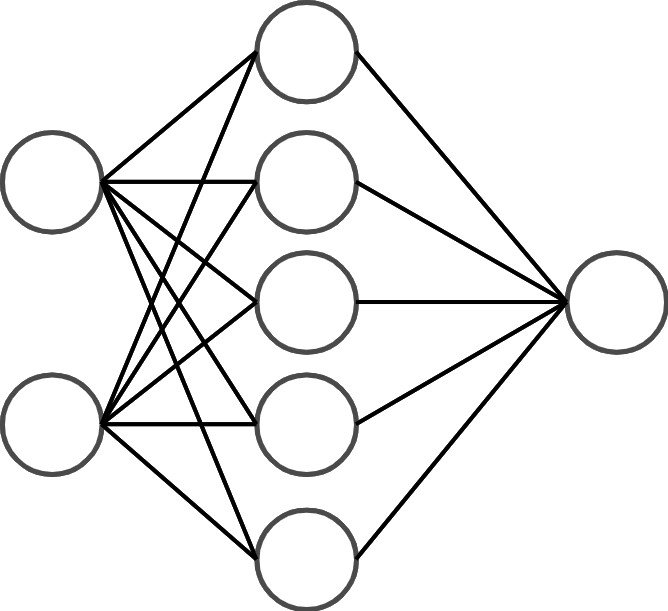
\includegraphics[width=0.5\textwidth]{Resultados/imgs/RedTF.png}
    \caption{Red neuronal implementada en Tensor Flow.}
    \label{fig:RedTF}
\end{figure}

Para la implementación con la biblioteca Tensor Flow se realizaron 1000 entrenamientos ya que esta es la cantidad máxima permitida por los recursos del hardware utilizado, con los resultados de estos entrenamientos se obtuvo el valor mínimo el valor máximo y el promedio de todos los experimentos.

\subsection{Carril central}

La Tabla \ref{tab:resultadosTFCCentral} muestra los resultados para el carril central en kilómetros por hora, podemos notar que para estos experimentos tenemos un promedio de 12.762 K/H con un valor mínimo de 1.872 K/H.


\begin{table}[H]
    \centering
    \caption{Resultados utilizando Tensor Flow Carril Central}
    \label{tab:resultadosTFCCentral}
    \begin{tabular}{|c|l|} \hline

    & \multicolumn{1}{c|}{\textbf{Error}} \\ \hline
    \textbf{MIN} & 1.872 \\ \hline
    \textbf{MAX} & 237.067 \\ \hline
    \textbf{Promedio} & 12.762 \\ \hline
    \end{tabular}
\end{table}


\subsection{Ultimo Carril}

La Tabla \ref{tab:resultadosTFCUltimo} muestra los resultados para el ultimo carril en kilómetros por hora, la cual nos muestra un valor mínimo de 2.128 K/H con un promedio de 13.172 K/H.


\begin{table}[H]
    \centering
    \caption{Resultados utilizando Tensor Flow Ultimo Carril}
    \label{tab:resultadosTFCUltimo}
    \begin{tabular}{|c|l|}\hline

    & \multicolumn{1}{c|}{\textbf{Error}} \\ \hline
    \textbf{MIN} & 2.128 \\ \hline
    \textbf{MAX} & 253.930 \\ \hline
    \textbf{Promedio} & 13.172 \\ \hline
    \end{tabular}
\end{table}

